\chapter{基于近存计算模拟器的矩阵向量乘硬件优化}
本章主要是基于此前的软件优化中出现的硬件架构方面的痛点对UPMEM硬件本身做修改,使用的是基于UPMEM的周期精确模拟器PIMulator\cite{uPimulator},分别做两大硬件改动:1)给UPMEM增添查找表专用的硬件单元支持乘加操作;2)给UPMEM增添SIMD单元支持向量操作。基于这两大硬件改动修改软件算法观察GEMV算子表现,对UPMEM的硬件架构进行探究并给出未来发展建议。

\section{PIMulator简介}
PIMulator是一个UPMEM的周期精确模拟器\cite{uPimulator},它由两个关键组件组成,如图\ref{PIMulator}所示:一个是与UPMEM指令集架构(Instruction Set Architecture, ISA)兼容的软件编译工具链,以及一个经过真实UPMEM-PIM硬件交叉验证的硬件性能模拟器。

\begin{figure}[!htbp]
	\centering
    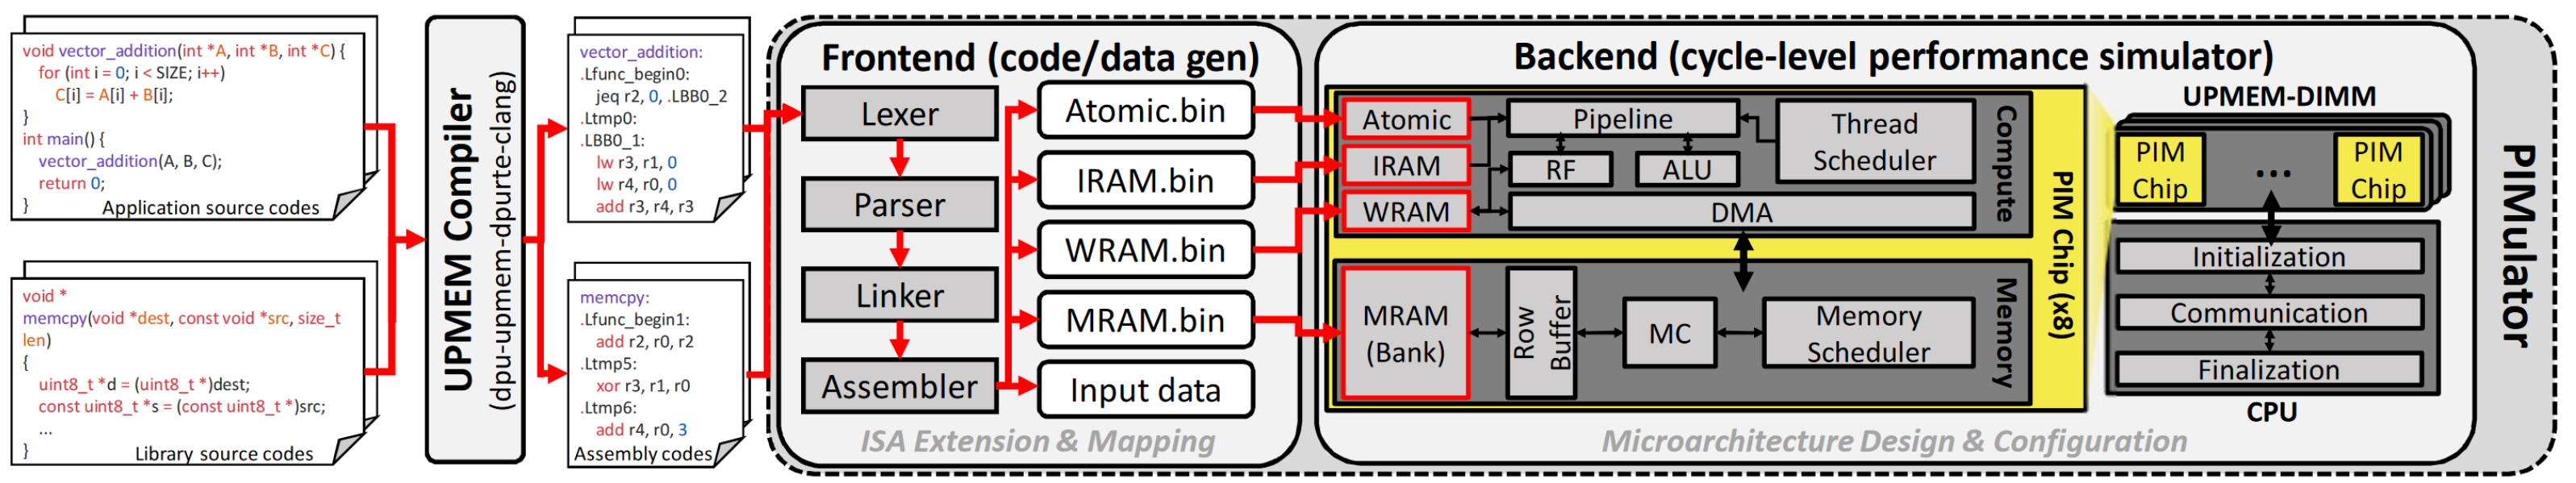
\includegraphics[width=0.9\textwidth]{figures/PIMulator.png}
	\caption{PIMulator架构图}
    \label{PIMulator}
\end{figure}

PIMulator的软件编译工具链的一部分基于开源的UPMEM软件开发工具包(Software Development Kit,SDK)提供的LLVM\cite{LLVM}编译器工具链(dpu-upmem-dpurte-clang),另一部分包括自定义的编译器、链接器和汇编器。PIMulator主要是用UPMEM SDK提供的编译器将用户所书写的能在真实硬件上运行的源代码以及和UPMEM兼容的C标准库程序进行预处理、编译和汇编成二进制对象,最终链接形成UPMEM的可执行二进制文件。同时,PIMulator使用自定义设计的链接器和汇编器,而不是直接使用UPMEM SDK的链接器。这是因为UPMEM的链接器与UPMEM硬件的微架构紧密绑定,限制了对PIM硬件架构的自定义能力。例如,当编译后的程序大小或WRAM内存使用量超过物理IRAM或WRAM容量时,UPMEM的链接器会报错。

PIMulator的硬件周期精确模拟器设计参考了UPMEM的用户手册和公开的微架构信息,主要设计点包括:1)对DPU计算核心进行建模:DPU核心被建模为一个14级顺序流水线处理器,充分模拟了流水线的调度算法以及奇偶寄存器堆访问时的限制。2)DRAM子系统建模:PIMulator的DRAM子系统模拟基于GPGPU-Sim的周期级DRAM模拟\cite{GPGPU-Sim}。由于UPMEM-PIM的内存调度策略细节未公开,PIMulator采用了首行优先,先到先服务(First Row, First Come First Served,FR-FCFS)算法来调度内存事务。3)CPU-DPU通信:设定固定通信值来模拟CPU和DPU之间的通信延迟,其值通过UPMEM-PIM真实硬件的系统性的性能分析来调整。UPMEM使用Intel AVX指令进行CPU-DPU通信,PIMulator同样模拟了这种通信的不对称带宽特性。

PIMulator的设计采用了模块化结构,将SPMD的前端代码/数据生成与后端模拟器清晰分离,类似于 GPGPU-Sim的设计。这种设计使得PIMulator可以轻松扩展以模拟和评估新的软硬件架构。例如希望改动PIMulator的硬件,为某种计算提供相应指令,只需要在前端修改自定义的编译、链接和汇编的相关代码识别对应汇编指令,然后在后端模拟器中添加相应的指令处理逻辑即可。

PIMulator有多个版本的实现\footnote{模拟器开源仓库:https://github.com/VIA-Research/uPIMulator},在论文中实现的是前后端分离的单线程版,使用的Python实现前端,C++做硬件模拟后端,没有多线程支持,但它的平均模拟速率为3KIPS(千条指令每秒),与GPGPU-Sim相当,在这个版本中,由于UPMEM的当前编程模型以及其通信和同步原语的工作方式,DPU大多数情况下作为独立的处理器运行。PIMulator另有一版基于Golang开发的前后端一体的版本,充分利用多协程(coroutine)实现了模拟速度提8.5倍的提升并且内存占用减少7.5倍。

\section{查表专用FMA指令}
在矩阵乘法的计算中,能够观察到一个非常基本的操作:向量和矩阵的元素相乘再与结果向量中的元素相加,将这种乘加操作融合成为单个操作,称为融合乘加(Fused Multiply Add,FMA)操作。在许多AI加速芯片中都设计有MAC单元(multiplier-accumulator unit)支持FMA操作和指令,其中也包括Intel的CPU。将乘加操作融合成为一条指令的优势一方面在于能够使得指令数目减少,减少取指和译码的时间,另一方面就是能够设计专门的电路优化计算,减少消耗周期数,从而整体提高算术吞吐。

类似地,我们可以基于查找表为UPMEM增加LFMA(Look-up Fused Multiply Add,LFMA)单元,专门用于处理使用查找表代替乘法的FMA操作。同时,使用查找表查找元素时,需要先计算偏移,再去访存,会花费两条指令,由于UPMEM每个周期最多只能执行一条指令,这种计算偏移的开销不可忽略,因此也可以将这部分的计算融入LFMA指令当中,设计指令为\verb|LFMA add: reg, base: reg, offset: reg, ele_width: imm|执行的操作是\verb|add+=[base+offset*ele_width]|。但是由于某些情形下只需查表而无需算加法,因此再设计一个查表专用指令LWO(Load With Offset),类似的\verb|LFMA target: reg, base: reg, offset: reg, ele_width: imm|,执行的操作为\verb|target=[base+offset*ele_width]|。

\begin{figure}[htbp!]
	\centering
	\subfigure[原本汇编代码]{
		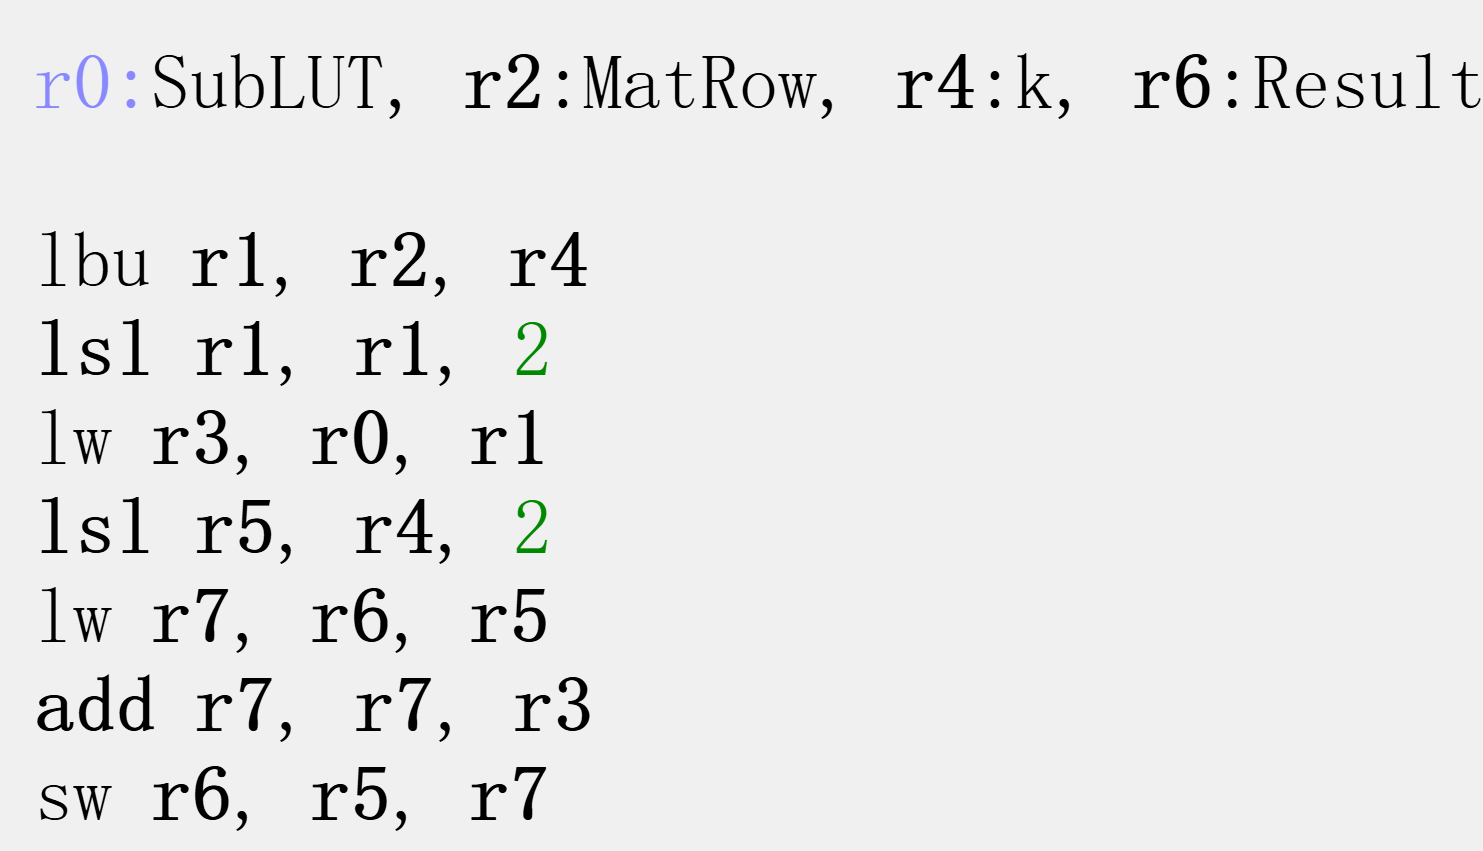
\includegraphics[width=0.4\textwidth]{figures/origin.png}
		\label{ASM:Before}}
	\subfigure[优化后汇编代码]{
		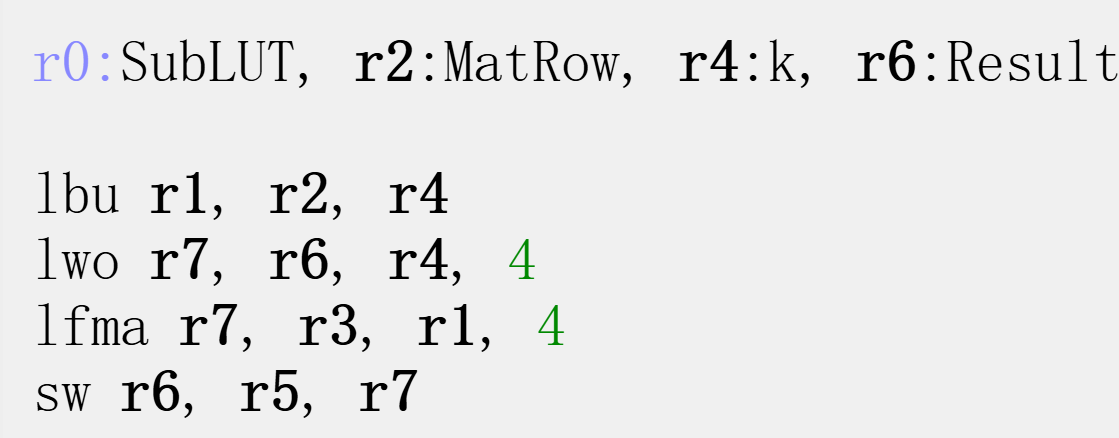
\includegraphics[width=0.5\textwidth]{figures/after.png}
        \label{ASM:After}}
	\label{ASM}
	\caption{查表专用指令汇编优化}
\end{figure}

如图\ref{ASM}所示,在算法\ref{LUT_Block}的最里层循环里,执行的计算为\verb|Result[k]+=SubLUT[Vector[j]&0xF][MatRow[k]];|,这个语句只有k在最内层循环发生改变,因此可以简化为\verb|Result[k]+=SubLUT[MatRow[k]];|可以看到,上述的语句的汇编中,查表SubLUT需要计算偏移因为查找表的每个元素是4字节,同样最后做累加时需要一起计算偏移做累加,因为结果向量的每个元素也是4字节。使用了LFMA和LWO指令后,指令数量从原本的7条减少到4条,性能几乎翻倍。

\section{基于SIMD指令查表的矩阵向量乘算法}
SIMD(Single Instruction Multiple Data)是一种特殊的计算模式,即“单指令多数据”,它允许处理器通过一条指令同时对多个数据执行相同的操作,从而显著提高数据处理的效率和性能。在SIMD架构中,处理器执行一条指令,但这条指令会同时作用于多个数据单元,同时执行相同的算术操作,因此SIMD指令非常适用于矩阵和向量的数据计算。Intel是SIMD计算模式的主要推动者,为多种架构的处理器配备了SIMD处理单元和对应的指令集\cite{IntelAVX},SIMD的数据位宽从一开始的128bit逐渐增长到256bit最后到521bit,大大提升了数据处理的效率。

对于更低bit量化的权重矩阵,我们可以为UPMEM增添SIMD指令进行加速。在Intel AVX-512指令中,有如下重排指令:\verb|__m512i _mm512_permutexvar_epi32(__m512i index, __m512i a)|,它接受两个AVX-512向量,并返回一个AVX-512向量,这些AVX-512向量由16个32位整形数组成,这个函数的作用是:按照index向量中指示的索引将a向量重排,比如index向量中第1个元素值是3,表示会将a向量中第4个元素重排到新向量的第1个位置。值的注意的是index向量中每个int32只用到了最低4bit的数值(确保索引值不超过16)。这种重排与查表操作存在相同之处,查表本身也是给出一张向量(子查找表),读取权重矩阵元素的值作为索引,再去查找表中取得乘积。上述函数中a向量为子查找表,权重矩阵的一行的前16个元素为index向量,相当于使用权重矩阵的值对子查找表做重排,可以一次性查出16个乘积结果。假设权重矩阵数据宽度为4bit,输入向量仍然是8bit的位宽,那么查找表为$256\times 16$的二维数组,仍然展开FP8到int32,那么LUT的每一行就是一个AVX512向量,刚好满足上述指令的条件。

要想使用SIMD计算GEMV,首先需要对权重矩阵进行重新划分,对于行主存的矩阵,现将其切分成$8\times 16$的子块SubMat如图\ref{SIMD},对这个子块我们对其进行重排,将其转换成一个AVX-512向量:将该AVX-512向量分组,分为16组INT32,将$\text{SubMat[0][0]}$的元素放置到INT32-0的最低四位$[0:4)$,再将$\text{SubMat[1][0]}$的元素放置到INT32-1的$[4:8)$,依次类推,直至遍历完8行,这样我们就填满了INT32-0,同样的道理,处理SubMat矩阵的第二列,得到INT32-1,当处理完SubMat的所有行和所有列之后,填满了该AVX-512向量。将该向量代替原子矩阵进行存储。完成了所有子块的重排之后,矩阵划分结束,其结果是行数减小到原来的8倍,列数扩大到原来的8倍。这时由于执行的是$8bit\times 4bit$的乘法,查找表的大小为$256\times 16\times 4Byte=16KB$,可以完全载入WRAM,因此可以直接按照GEMV内积的方式计算。

\begin{figure}[!htbp]
	\centering
    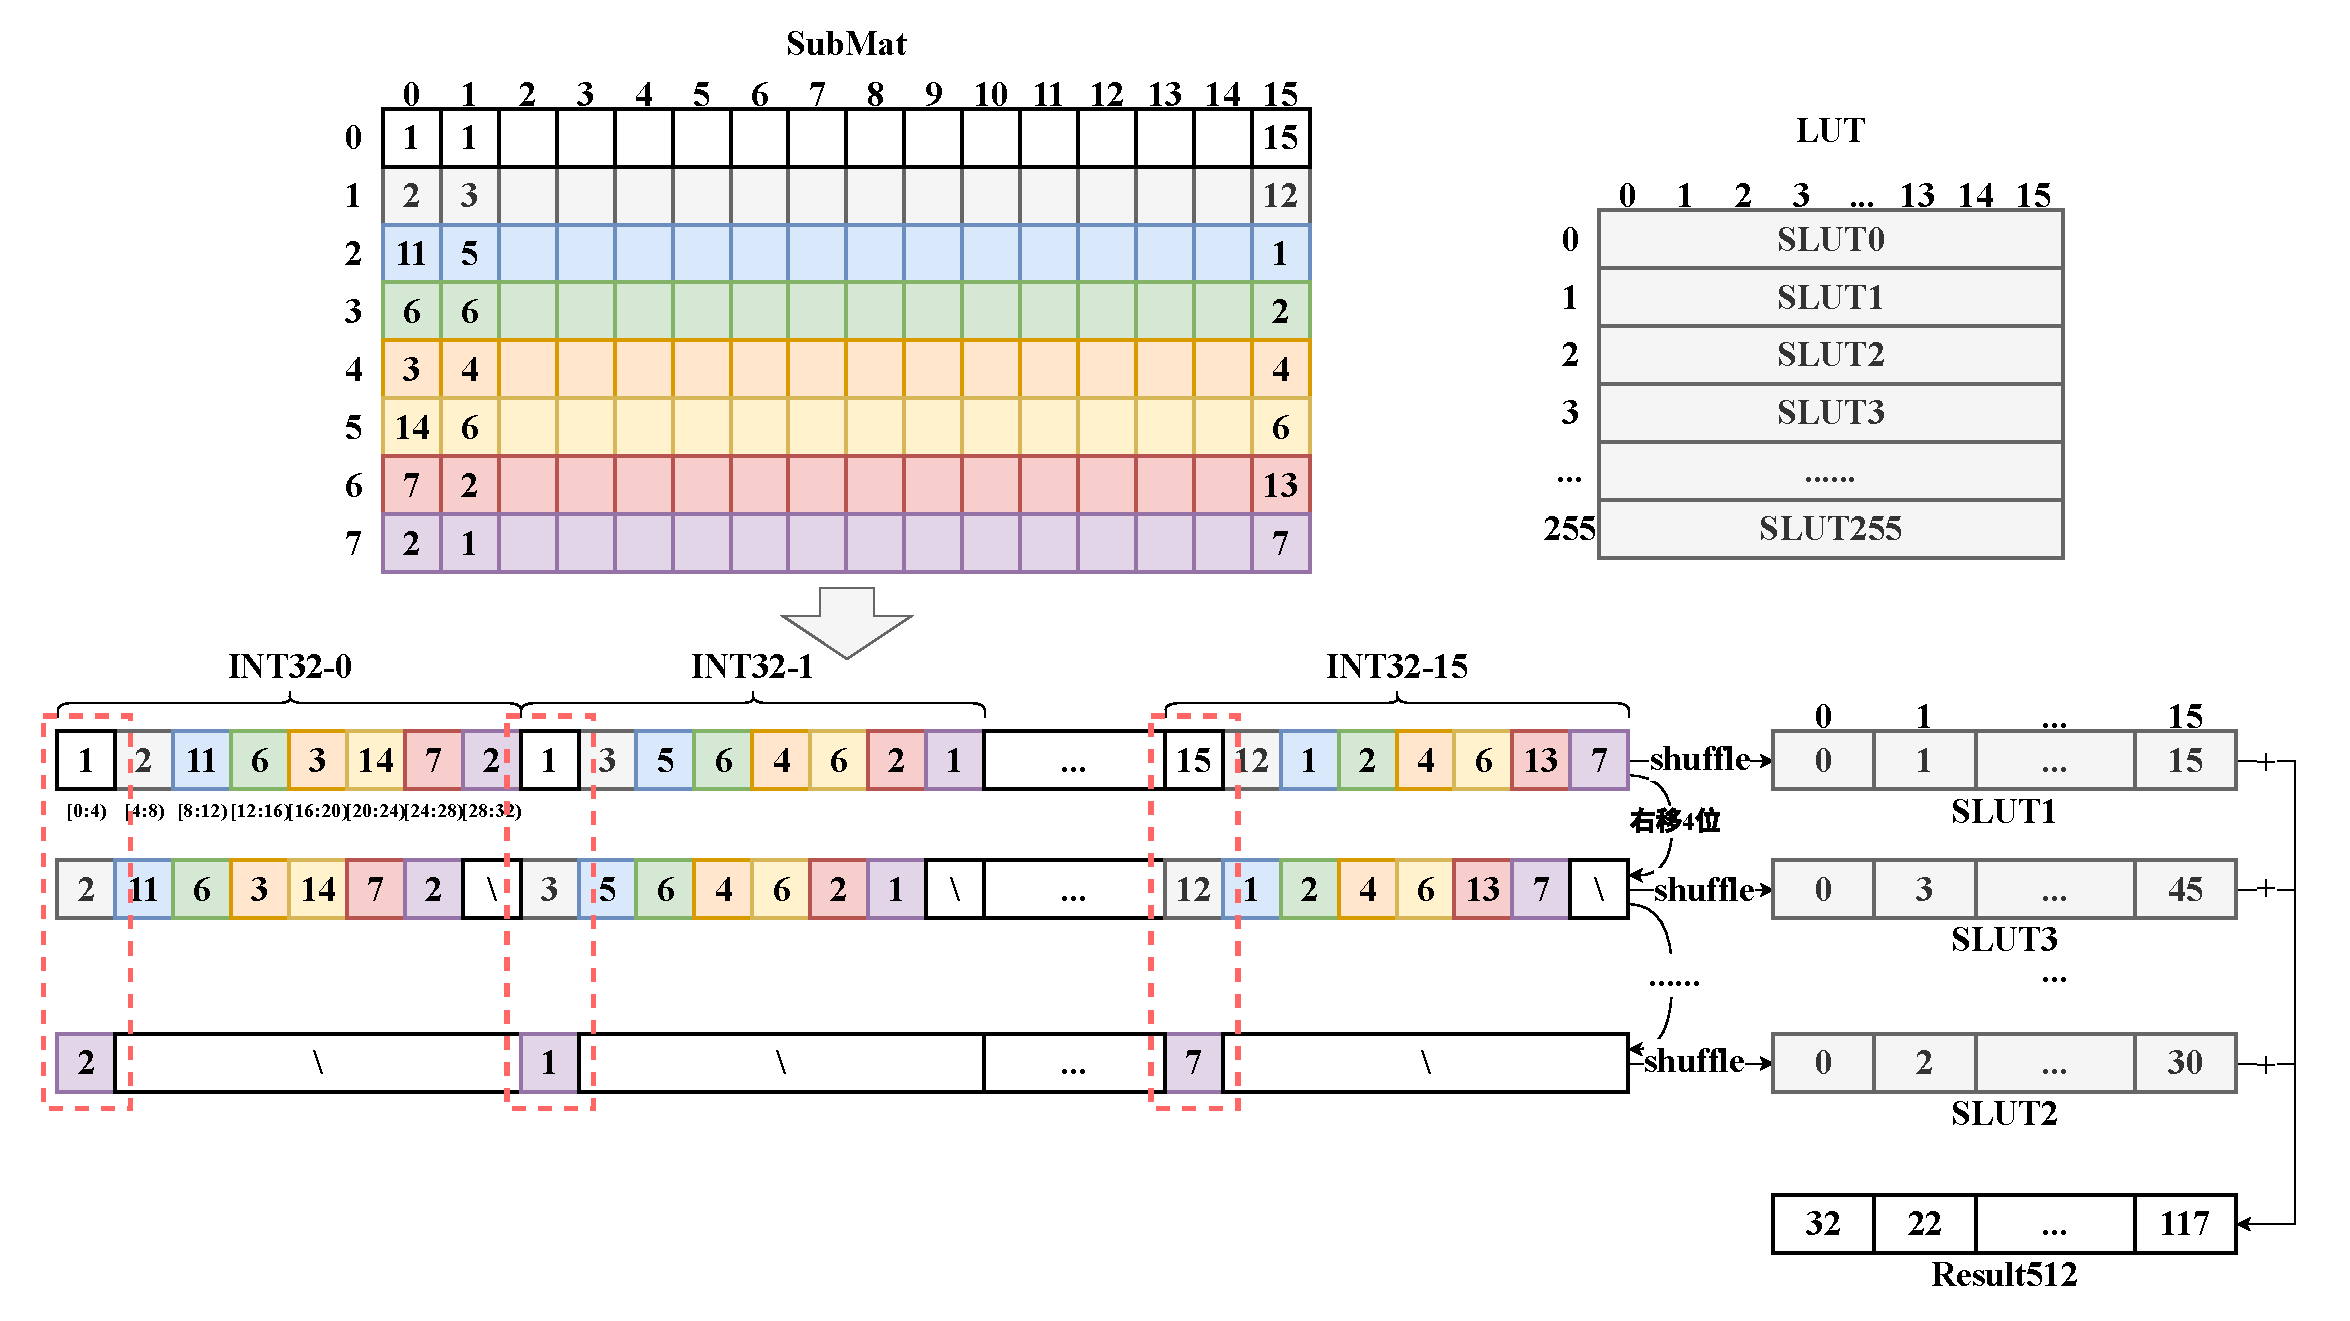
\includegraphics[width=0.9\textwidth]{figures/SIMD.pdf}
	\caption{使用SIMD重排指令的矩阵构建和计算示意图}
    \label{SIMD}
\end{figure}

具体的计算方式也需要将重排后的权重矩阵从行主存改为列主存,也就是以512bit的粒度进行转置。转置过后,原来一列的元素现在可以按照行访问提高访问效率,再并行化,每个tasklet处理一列。具体到单个AVX-512向量计算仍然以图\ref{SIMD}为例,计算该AVX-512向量时需要先载入对应的子查找表SLUT1,载入该行子查找表到AVX-512向量a中(使用\verb|_mm512_loadu_si512|指令载入寄存器),然后载入该AVX-512向量到index中,执行\verb|_mm512_permutexvar_epi32|操作得到结果向量,使用\verb|_mm512_add_epi32|指令将其加到累加AVX-512结果寄存器上。然后使用\verb|_mm512_srli_epi32|指令对index向量右移4位,再重复刚才的过程;左移8次后完成整个AVX-512向量的计算,再类似依次执行该列的所有AVX-512向量的计算,执行完成后再将AVX-512的累加寄存器写到结果向量的对应位置上。不同的tasklet负责不同的列,其对应的结果向量的位置也不同,但是之间互相不干扰无竞争。

要想完成上述工作,需要给UPMEM增加相应的向量单元并适配相应的指令集,除了需要之前介绍的\verb|_mm512_permutexvar_epi32|指令的支持之外,还需要引入一些新的指令,比如\verb|_mm512_loadu_si512|指令用于载入AVX-512向量,\verb|_mm512_add_epi32|指令用于向量加法运算,\verb|_mm512_srli_epi32|指令用于右移运算,\verb|_mm512_storeu_si512|指令用于将AVX-512向量存储到内存中。同时要高效完成上述工作,每个线程至少需要4个AVX-512寄存器,其中两个分别充当a和index,剩下的两个一个用于暂存向量重排的结果,一个用作累加寄存器。我们将这些指令和寄存器通过PIMulator加到UPMEM的软硬架构中,根据Intel AVX-512指令手册设置运算的每指令周期数(Cycle Per Instruction,CPI),都设置成1个时钟周期。

\section{本章小结}